\documentclass[lettersize,journal]{IEEEtran}
\usepackage{amsmath,amsfonts}
\usepackage{algorithmic}
\usepackage{algorithm}
\usepackage{array}
\usepackage[caption=false,font=normalsize,labelfont=sf,textfont=sf]{subfig}
\usepackage{textcomp}
\usepackage{stfloats}
\usepackage{url}
\usepackage{verbatim}
\usepackage{graphicx}
\usepackage{cite}
\usepackage{wasysym}
% \setmathfont{XITS Math}
% updated with editorial comments 8/9/2021

\begin{document}

\title{MAE 298 Introduction to PDEs \\ Electrochemical Modeling of Batteries}

\author{Jonathan Dorsey}


% Remember, if you use this you must call \IEEEpubidadjcol in the second
% column for its text to clear the IEEEpubid mark.

\maketitle

\begin{abstract}
This
\end{abstract}

\section{Introduction}
\IEEEPARstart{P}{artial} differential equations (PDEs) provide a the mathematical basis for describing a significant number of scientific pheonimon; however, while the study of PDEs is import, it can often be more challenging to develope PDE which models these phenomina from first principles than it is to understand the structure of a given PDE. This can be more readily seen when investigating more complex systems which couple several PDEs together to describe the full dynamics of the system. To this point, electrochemical models of lithium-ion batteries fall into this category of complex systems. Even simple electrochemical models of batteries consist of anywhere upto five PDEs. The objective of this paper will be to derive the salient PDEs describing the electrochemical battery model known as Doyle-Fuller-Newman (DFN) model, with enough context and background about the first principles being applied to enlighten the reader as to how and why the given PDE model is meaningful.

\section{Doyle-Fuller-Newman Model Overview}
The DFN model has long been held as the gold standard electrochemical battery model. This model describes at the microscale dynamics of a planar battery cell (SHOWN IN FIG) which has been volume averaged to account for usage of this model as a full battery cell, which accounts for behaviors such as mass and charge conservation, as well as the process of intercalation and deintercalation where lithium is distributing through the material of electrode material or coating during charging and discharging respectively. This model can be broken down in to the five following categories. In turn, this paper will investigate each category, and provide the context and first principles analysis which yield appropriate governing PDEs.

\begin{enumerate}
  \item
  \item
  \item
  \item

\end{enumerate}

\[
  \oiint x^2 +5
\]




\section{Microscale Model Derivation}

Before the complete Doyle-Fuller-Newman (DFN) model can be computed, it is neccessary to compute the microscale dynamics which govern the behavior of the compute electrochemical system. Only after this microscale model has been developed can we apply them to derving the complete DFN model. In the microscale model, the principle mechanisms of operation are evaluated under the assumtion of homogeneous materials. Under this assumption, the model does not account for individual molecular interactions or impurities. For this analysis, we can assume that these molecular inconistentcies averaged out to create a homogeneous material for which we can independently derive and evaluate the governing equations for both the solid and electroyte phases of the battery.



\subsection{Charge Conservation in Homogeneous Solid}

The first step in this model is to use the principle of conservation of charge, in the solid phase of the battery. This means that charge is not created or destroyed within the battery. The principle used to derive this equation is the point for of \textbf{Ohms Law}. This means that we assume that through the electrode material, electron movement is caused by drifting of charge, as perscribed by Ohms Law. Namely...

\[
\textbf{i} = \sigma\textbf{E}
\]

Where \textbf{i} is the current density [$Am^{-2}$], $\sigma$ is the conductivity of the electrode material, and \textbf{E} is the applied electric field. This is an alternate form of Ohms Law ($V = IR$)


\subsection{Mass Conservation in Homogeneous Solid}

The conservation of mass in homogeneous solid (electrodes) is used to capture the dynamics of lithium intercalation into the crystalline structure of the electrode materials. Specifically, Fick's first law is used to describe quanity of molar flux density \textbf{N} to the gradient of lithium concentration in the solid electrode material, where D is the material dependent diffusivity.

\[
\textbf{N} =  -D \nabla c
\]

This expression states that the magnitude of the lithium molar flux density will increase with an increase in the gradient of the concentration. From this expression, we can compute the net molar flux by computing the integral of the entire domain boundary.

\[
 j = -\iint_{S} \textbf{N} \cdot \hat{\textbf{n}}dS
\]

This is equivalent to the statement that ...

\[
j = \frac{dn}{dt}
\]

Where n is the number of moles. Furthermore, we can define $dn$ as a function of concentration. This expression can be computed by integrating each contribution of concentration within a differential volume over the entire volume of the domain.

\[
dn = d \iiint_V cdV
\]

By applying this substition and then and equating the net molar flux densities, we find that...

\[
\iint_S \textbf{N} \cdot \hat{n}dS = -\frac{d}{dt} \iiint_V c dV
\]

This expression if the integral form of the continuity equation. The take away from this equation is that no mass has been created or destroyed inside the domain. Also this implies that all mass transfer which does occur happens only at the boundaries of the domain.

By further massaging and manipulating the previous equation, we can reduce this equation into the more familiar form of Fick's second law, as shown below.

\[
\frac{\partial c_{S}}{\partial t} = \nabla \cdot \left( D_{S} \nabla c_{s} \right)
\]

The intuition behind this law is that it encapsulates the dynamic relationship between the concentration as it changes in time to the concentration as it changes in space.


\subsection{Charge Conservation in Homogeneous Electrolyte}

When discussing the conservation of charge inside of the electrolyte phase of the battery, a non-trivial amount of thermodynamics and physical chemistry are required to fully contextualize the groundwork which needs to be laid, to understand the principles for deriving the governing equations. Without diving extremely deep into these areas, it is useful to have a basic explaination about how these concepts are linked.

\subsubsection{Gibbs Free Energy}
A simple definition of Gibbs Free Energy is that it is the amount required to create the system (internal energy u), plus the amount which boundary work (pV) required to make room for the system, minus the energy which is obtained from the surrounding environement (TS), which has a temperate of T. This can be written...

\[
    G = U + pV - TS
\]

 The \textbf{free energy} portion of the name, is important because it informs us of how much energy can be extracted from the system, so long as the temperature and pressure are held constant. Additionally, the sign of the Gibbs free energy dictates the direction that a chemical reaction will spontaneously take. \\

 In the context of batteries, Gibbs free energy is used in the formulation of electrochemical potentials, which are discussed below.


 \subsubsection{Molarity \& Molality}

 Since an electrolyte is a solution, it can be described as an intensive property via its molarity and molality, depending on which attributes of the solution are of interest.

 The molarity of a solution is defined to be the number of moles of solute per liter of solution.

 \[
    c_i = \frac{n_{solute_i}}{V_{solution}}
 \]

 Where as the molality of the solution, is defined to be the total number of moles of solute over the mass of the solvent.

 \[
    m_i = \frac{n_{solute_i}}{m_{solvent}}
 \]


 \subsubsection{Electrochemical Potential}

 Understanding the previous sections is important because it leads to a discussion of electrochemical potentials. Especially in multispecies solutions, the conversion from extensive properties to intensive properties is subtle. In order to property define these intensive properties, it is neccessary to define partial molar quanities. This can be written using partial derivatives and describes how much the Gibbs free energy (extensive) changes with the addition of only species to the solution. This can be written...

 \[
    \bar{\mu} = \left( \frac{\partial G}{\partial n_{i}} \right)_{T,p,n_{j} (j \neq i)}
 \]

 where $n_i$ is the number of moles of species $i$, while keeping the temperature, pressure, and moles of other species constant. As can be seen by the equation, the electrochemical potential is an intensive property which has been normalized via the species mass (in moles).

 By applying this operator to the Gibbs free energy we can see that there will be some amount of internal potential as well as an external potential which contributes to the total electrochemical potential of the system.

\[
    \bar{\mu_{i}} = \bar{\mu}_{i, internal} + \bar{\mu}_{i, external}
\]

 In the absense of other potentials and forces from external fields, the effect of chemical and electrochemical potentials can be written as ...

 \[
    \bar{\mu}_{i} = \mu_{i} + z_i F \phi
 \]


Where the $z_i$ is the charge number, $F$ is Faraday's constant, and $\phi$ is the local electrostatic potential. After applying Euler's theorem for homogeneous functions we can show

\[
    G(\textbf{n}) = \textbf{n} \cdot \nabla G (\textbf{n}) = \sum_i n_i \frac{\partial G}{\partial n_i}
\]

\[
    G = \sum_i n_i \bar{\mu}_i
\]

This provides a very concise form for replacing Gibbs free energy with electrochemical potentials

\subsubsection{Gibbs-Duhem Equation}

This equation provides relationship between electrochemical potentials, which reduces the number of simultaneous equations which we must solve.

\[
    G = U + pV - TS
\]

\[
    dG = dU = d(pV) - d(TS)
\]

\[
        = dq + dw + pdV + VdP -TdS - SdT
\]

From thermodynamics we know $dw = -pdV$ and that under the assumption of reversibility $dq = TdS$ that we obtain...

\[
    dG = Vdp - SdT
\]

We can show from the previous relationship relating Gibbs free energy and electrochemical potential that...

\[
    \sum_{r}^{i=1} n_id\bar{\mu}_i = Vdp - SdT
\]

such that....

\[
    \sum_{i=1}^{r} n_id\bar{\mu}_i - Vdp + SdT = 0
\]

In the special case we are interested in (a binary electrolyte) containing only two species, this equation can be explicitily written as

\[
    n_1 d\bar{\mu}_1 + n_2 d\bar{\mu}_2 = 0
\]


It should be noted that this equation is only valid under the isothermal and isobaric process. However given that we are operating under these assumptions, then we can see the relationship between the two electrochemical potentials. If one is increased, the other must decrease to maintain the equality. In the general case...

\[
    \sum_{i=1}^{r} c_{i}d\bar{\mu}_i = 0
\]

It should also be noted that we can easily convert this from molar to molarity by dividing by the volume. \\

\subsubsection{Activity}

Unlike non-ionic solutions, ionic solutions do not distribute their ions randomly, this is because the electrical charge for either a cation or anion are preferentially oriented and attracted to ions of the opposite charge. A consequence of this behavior is that movement of ions in solution are artificially slow, due to the movement of a specific ion also attempting to drag the other ions which are in its immediate neighborhood in the solution. \\

Because of this phenomenon, we can use the \textbf{activity} of a species as an effective concentration, which accounts for this descrepency.

\[
    a_i = c_i f_i
\]

In the context of lithium-ion batteries, the concept of activity is important because the transport medium between each electrode is a neutral ionic solution, which has a fixed number of positive and negative charge carries, that faciliate transfer of charge inside the battery. Therefore modeling this non-intutiative behavior is an important step in capturing the complete dynamics at play.

\subsubsection{ Stoichiometric Coefficient $\nu$ }
In a balanced chemical equation, the total amount of matter (of each element/molecule) and the total amount of charge are conserved. This fact holds true for electrolytes. In the case of an electrolyte, the solution is comprised of solute dispursed throughout a solvent such that the overall solution is charge-neutral. An example is shown below.

\[
\mathrm{Na}_{2} \mathrm{SO}_{4} \rightarrow 2 \mathrm{Na}^{+}+\mathrm{SO}_{4}^{2-}
\]

In this example, the coefficents in from of each ion on the right-hand-side of the equation, are known as \textbf{stoichiometric coefficients}, and are denoted with the symbol $\nu$. In the equation shown above, the stoichiometric coefficents are $\nu_{Na^{+}} = 2$ and $\nu_{SO_{4}^{2-}} = 1$.

\subsubsection{ Charge Number }

Similar to the stoichiometric coefficents, the \textbf{charge number} is also displayed in the chemical equation, as the super-script for each compound on the right-hand-side of the the balanced chemical equation. The charge number tells us how many excess electrons or protons exist in each given ion compound. The charge numbers for the equation above are $z_{Na^{+} = 1}$ and $ z_{SO_{4}^{2-}} = -2 $. The sign of the charge number informs us whether each compound is a cation ($z>0$) or anion ($z < 0 $)

\subsubsection{ Electroneutrality in Binary Electroytes }
As mentioned previously electroneutrality is an important and frequently referenced concept in the developement of the equations. In particular, a binary electrolyte comprised of only species is of particular interest and has useful properties which are very relavent to lithium-ion battery models. Under the constraint of charge-neutrality, we can state that the net charge in the solution must be $q = 0$. This can be expressed via charge numbers and the stoichiometric coefficents described above as follows.

\[
\sum_{i} z_{i} v_{i}=0
\]

For the general case the subscripts indicated whether the charge is from a cation or an anion, or the contributions form the solvent.
\[
z_{+} v_{+}+z_{-} v_{-}+z_{0} v_{0}=0
\]

However, since the solvents in the electroyte are always charge neutral, we can ommit them from this equation, leavinging the following expression.

\[
z_{+} v_{+}+z_{-} v_{-}=0
\]

\[
\frac{c_{+}}{v_{+}}=\frac{c_{-}}{v_{-}}
\]


\subsubsection{ Deriving Current Flow }

\subsubsection{ Deriving Conservation of Charge }

\[
\frac{\partial c_{i}}{\partial t}=-\nabla \cdot \mathbf{N}_{i}+R_{i}
\]


\[
F \frac{\partial z_{i} c_{i}}{\partial t}=-\nabla \cdot\left(z_{i} F \mathbf{N}_{i}\right)+z_{i} F R_{i}
\]


\[
\frac{\partial}{\partial t} F \sum_{i} z_{i} c_{i}=-\nabla \cdot\left(F \sum_{i} z_{i} \mathbf{N}_{i}\right)+F \sum_{i} z_{i} R_{i}
\]

\[
\frac{\partial}{\partial t} F \sum_{i} z_{i} c_{i}=-\nabla \cdot\left(F \sum_{i} z_{i} \mathbf{N}_{i}\right)
\]

\[
\nabla \cdot \mathbf{i}=0
\]














\subsection{Mass Conservation in Homogeneous Electrolyte}

\[
\mathbf{v}_{1}^{\prime}=\frac{m_{1} \mathbf{v}_{1}+m_{2} \mathbf{v}_{2}}{m_{1}+m_{2}}
\]

\[
\begin{aligned}
\Delta\left(m_{1} \mathbf{v}_{1}\right) &=m_{1}\left(\mathbf{v}_{1}-\mathbf{v}_{1}^{\prime}\right) \\
&=m_{1}\left(\mathbf{v}_{1}-\frac{m_{1} \mathbf{v}_{1}+m_{2} \mathbf{v}_{2}}{m_{1}+m_{2}}\right)
\end{aligned}
\]

\[
=\frac{m_{1} m_{2}}{m_{1}+m_{2}}\left(\mathbf{v}_{1}-\mathbf{v}_{2}\right)
\]

\[
\left(\frac{\mathrm{dp}}{\mathrm{d} t}\right)_{V}^{\text {species- }} \propto c_{1} c_{2}\left(\mathbf{v}_{1}-\mathbf{v}_{2}\right)
\]

\[
C_{T}=\sum_{i} c_{i}
\]

\[
x_{i}=\frac{n_{i}}{n}=\frac{n_{i} / V}{n / V}=\frac{c_{i}}{c_{T}}
\]

\[
\left(\frac{\mathrm{d} \mathrm{p}}{\mathrm{d} t}\right)_{V}^{\text {species- }} \propto x_{1} x_{2}\left(\mathrm{v}_{1}-\mathrm{v}_{2}\right)
\]

\[
\mathrm{F}_{1, \mathrm{~V}} \propto x_{1} x_{2}\left(\mathrm{v}_{1}-\mathrm{v}_{2}\right)
\]

\[
% \mathscr{D}_{i j}=\frac{x_{i} x_{j}}{K_{i j}} p
\]

\[
% K_{i j}=\frac{R T c_{i} c_{j}}{c_{T} \mathscr{D}_{i j}}
\]

\[
\mathrm{F}_{1}=-\nabla G_{1}=-\frac{\partial G_{1}}{\partial \mu_{1}} \nabla \bar{\mu}_{1}=-n_{1} \nabla \bar{\mu}_{1}
\]

\[
\mathrm{F}_{1, V}=\frac{\mathrm{F}_{1}}{V}=-\frac{n_{1}}{V} \nabla \mu_{1}=-c_{1} \nabla \beta_{1}
\]






\[
\frac{\partial c}{\partial t}=\nabla \cdot\left[D\left(1-\frac{\mathrm{d} \ln c_{0}}{\mathrm{~d} \ln c}\right) \nabla c\right]-\frac{\mathbf{i} \cdot \nabla t_{+}^{0}}{z_{+} v_{+} F}-\nabla \cdot\left(c \mathbf{v}_{0}\right)
\]



\subsection{Lithium Movement Between Solid \& Electrolyte Phases}


\section{DFN Model Derivation}

The previous system of governing partial differential equations, was derived using the microscale interactions and mechanisms. While this approach to analysis is particularly informative about the how these sorts of high fidelity models are derived, solving them for an entire cell (using a system of thousands or millions of coupled PDEs) is computationally infeasible, even for modern computers. There are many different approaches to creating macroscale models that capture the first principle mechanisms of action, but are far more computationally viable. This simplification comes with a penalty on the accuracy of model; however, these models are still far and away some of the most high fidelity battery models which are routinely used today to check  \\

In particular, the Doyle-Fuller-Newman (DFN) model uses a technique of volume averaging to be able to same governing equations which were derived above, over larger domains, approximating (on average) the behaviors of each electrode and the electrolyte. \\

\subsection{Volume Averaging Methods}

\section{Single Particle Model (SPM \& SPMe)}

\section{Analysis of Governing Equations}

\section{Numerical Solution}

\section{Results}

\section{Conclusion}
The conclusion goes here.


\section*{Acknowledgments}
This should be a simple paragraph before the References to thank those individuals and institutions who have supported your work on this article.

\section{References Section}
You can use a bibliography generated by BibTeX as a .bbl file.
 BibTeX documentation can be easily obtained at:
 http://mirror.ctan.org/biblio/bibtex/contrib/doc/
 The IEEEtran BibTeX style support page is:
 http://www.michaelshell.org/tex/ieeetran/bibtex/

 % argument is your BibTeX string definitions and bibliography database(s)
%\bibliography{IEEEabrv,../bib/paper}
%
\section{Simple References}
You can manually copy in the resultant .bbl file and set second argument of $\backslash${\tt{begin}} to the number of references
 (used to reserve space for the reference number labels box).

\begin{thebibliography}{1}
\bibliographystyle{IEEEtran}

\bibitem{ref1}
{\it{Mathematics Into Type}}. American Mathematical Society. [Online]. Available: https://www.ams.org/arc/styleguide/mit-2.pdf

\bibitem{ref2}
T. W. Chaundy, P. R. Barrett and C. Batey, {\it{The Printing of Mathematics}}. London, U.K., Oxford Univ. Press, 1954.

\bibitem{ref3}
F. Mittelbach and M. Goossens, {\it{The \LaTeX Companion}}, 2nd ed. Boston, MA, USA: Pearson, 2004.

\end{thebibliography}


\newpage

\section{Biography Section}

\vspace{11pt}

% \bf{If you include a photo:}\vspace{-33pt}
% \begin{IEEEbiography}[{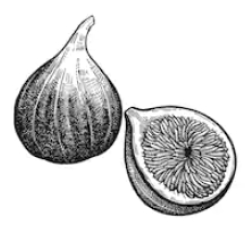
\includegraphics[width=1in,height=1.25in,clip,keepaspectratio]{fig1}}]{Michael Shell}
% Use $\backslash${\tt{begin\{IEEEbiography\}}} and then for the 1st argument use $\backslash${\tt{includegraphics}} to declare and link the author photo.
% Use the author name as the 3rd argument followed by the biography text.
% \end{IEEEbiography}

\vspace{11pt}

\vfill

\end{document}
